\section{Rendering System}
\subsection{Introduction}
The rendering system is a key component of the Volumetric Simulator, responsible for displaying models in a manner that makes them appear three-dimensional. It needs to be fast and responsive to maintain the illusion of 3D.

\subsection{OpenGL}

Our project requires the rendering system to render 3D models in real-time with low latency and a high frame rate. We decided to use OpenGL \cite{woo1999opengl} to achieve this due to its low-level control over the rendering pipeline and cross-platform compatibility. \\

We briefly considered using fully fledged game engines like Unity \cite{noauthor_unity_nodate} or Unreal Engine \cite{unrealengine}, but ultimately decided against them due to the significant overhead and lack of fine control over the rendering pipeline. Additionally, we utilised the OpenGL-compatible GLM \cite{noauthor_g-trucglm_2024} mathematical library for matrix manipulation and projections, as it was sufficiently fast and simple to use.

\subsection{Perspective}

As covered extensively in the background section, the user’s perspective is crucial for creating the illusion of 3D. To achieve this, we used positions provided by the tracking system to calculate the correct dimensions for the viewing frustums, rendering the scene from the user’s perspective. The results of this method, used to render a chessboard, can be seen in Fig.~\ref{fig:right-view} and Fig.~\ref{fig:left-view}.

\begin{invisBox}
	\pictureBox[label={fig:right-view}]{Right Perspective}{
		\adjustbox{height=5.75cm, keepaspectratio}{
			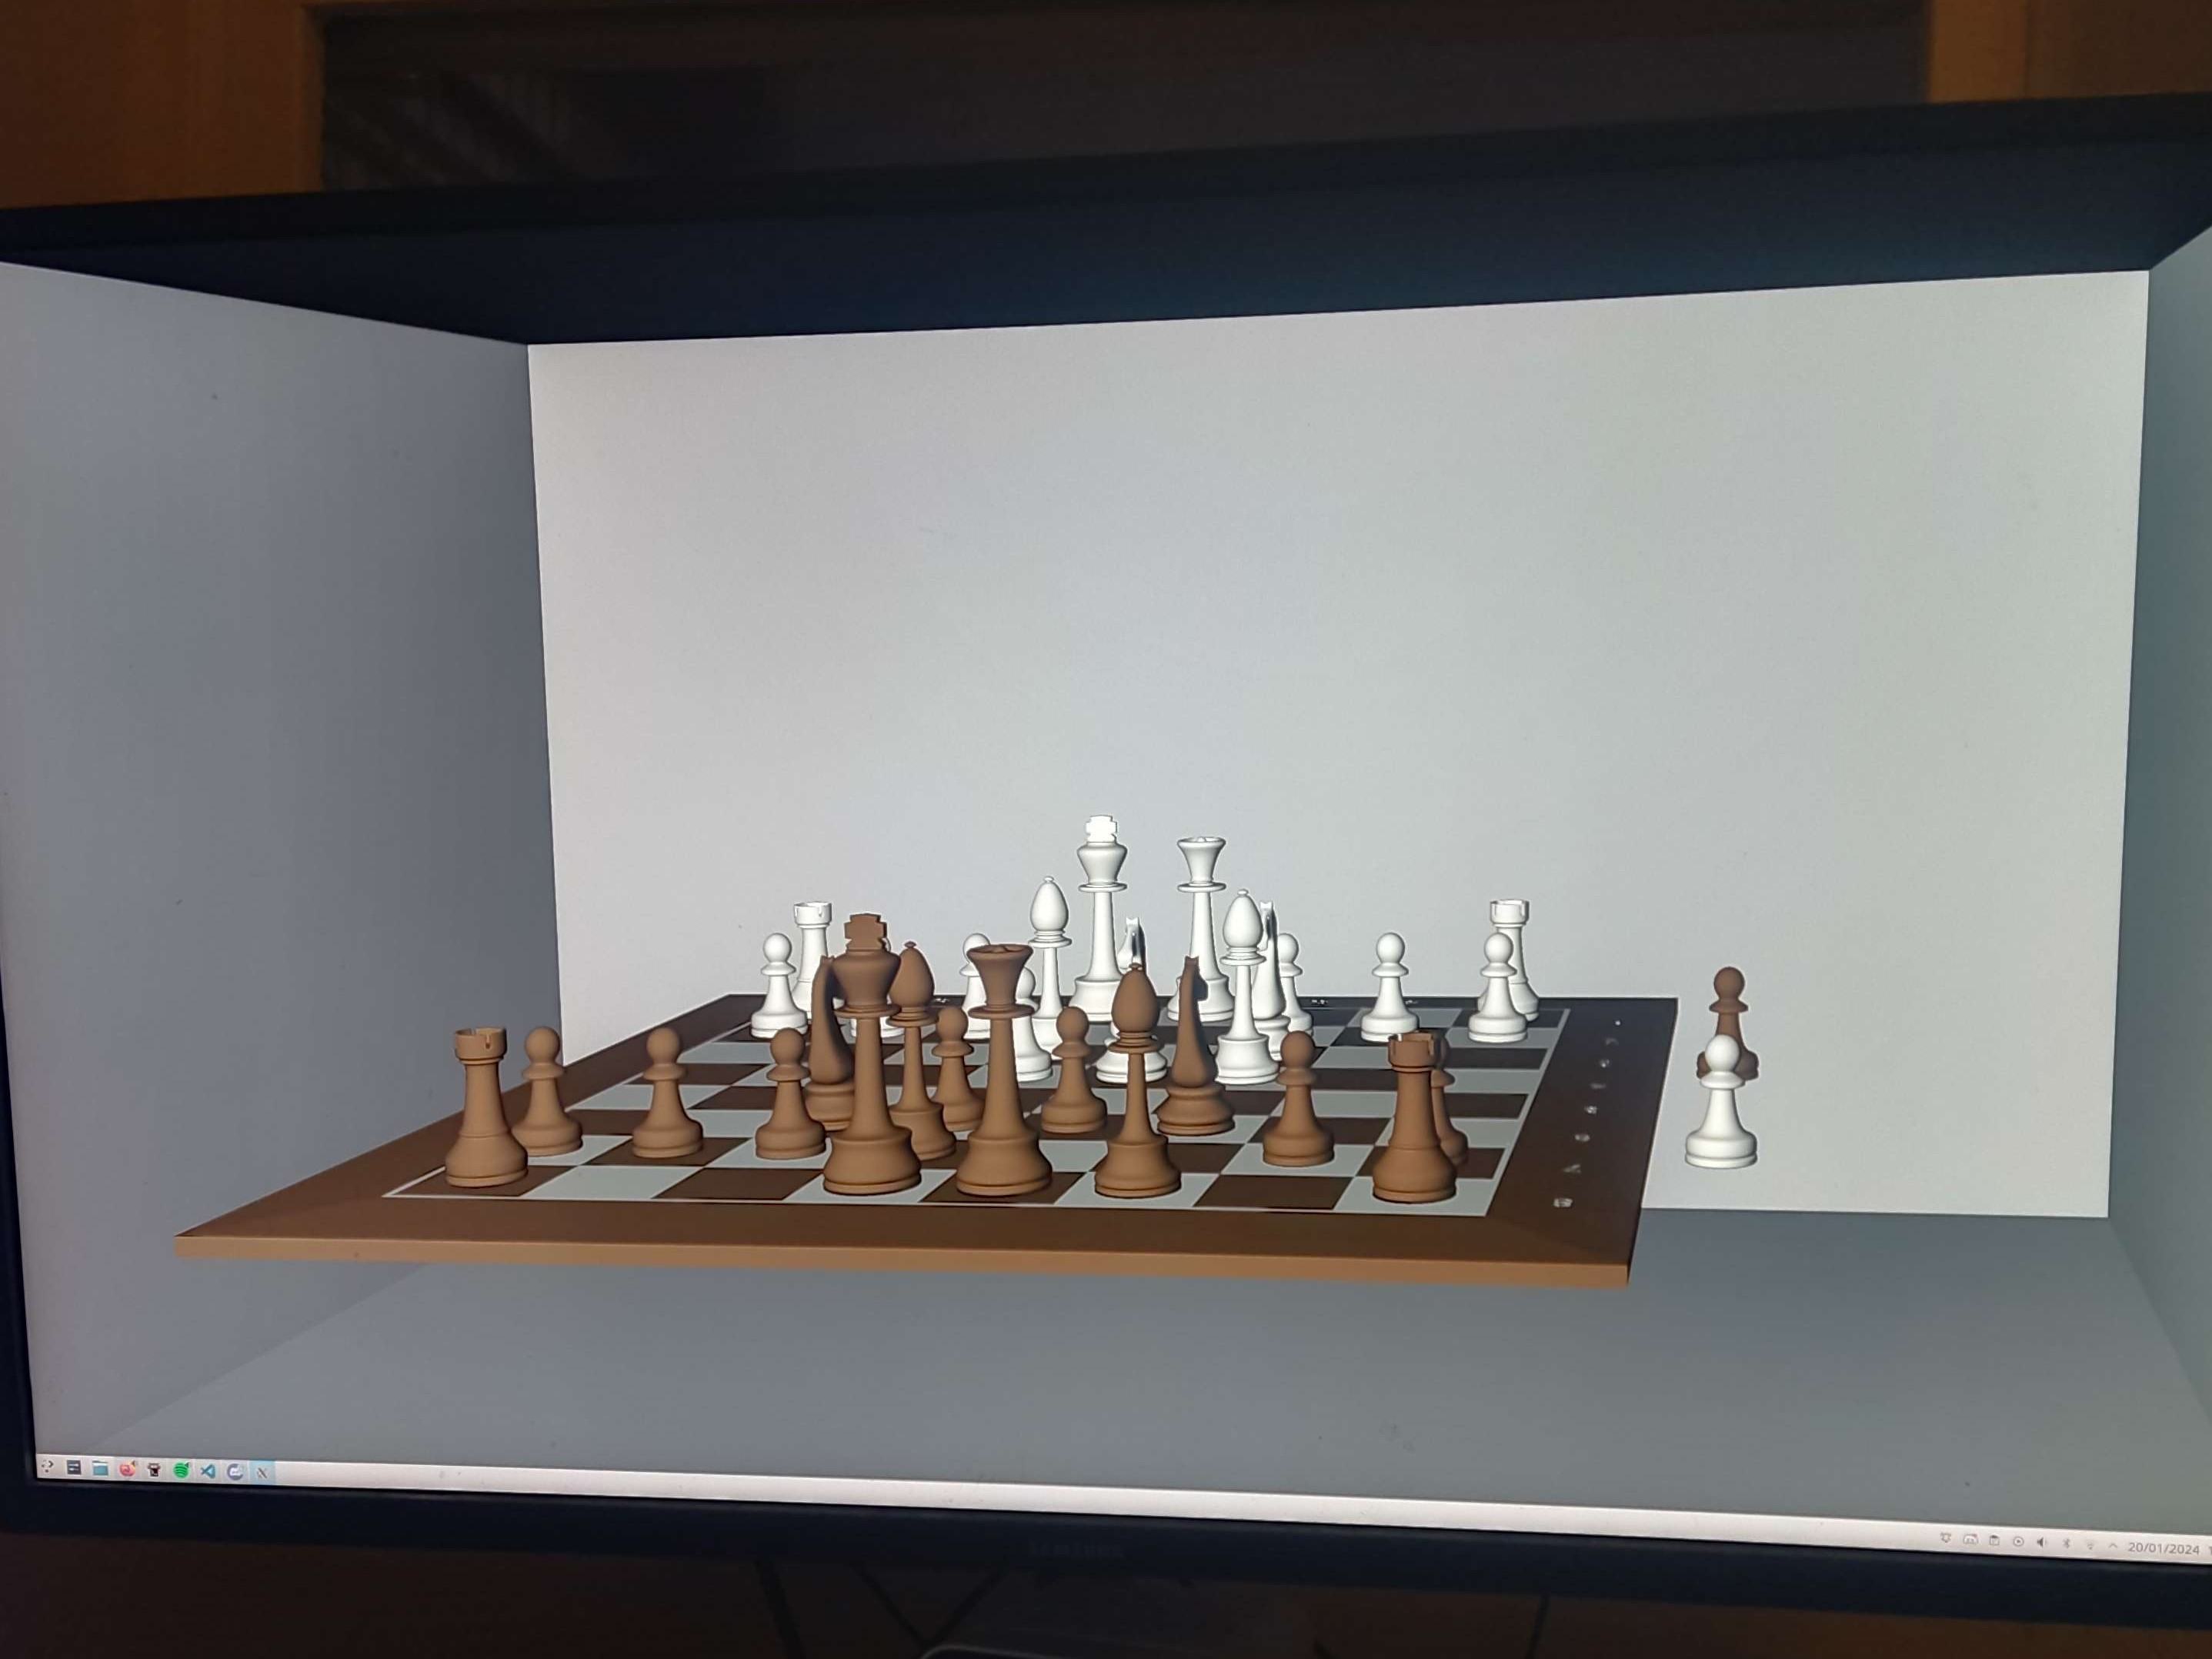
\includegraphics{./implementation/figures/perspective/right.jpg}
		}
	}
	\hfill
	\pictureBox[label={fig:left-view}]{Left Perspective}{
		\adjustbox{height=5.75cm, keepaspectratio}{
			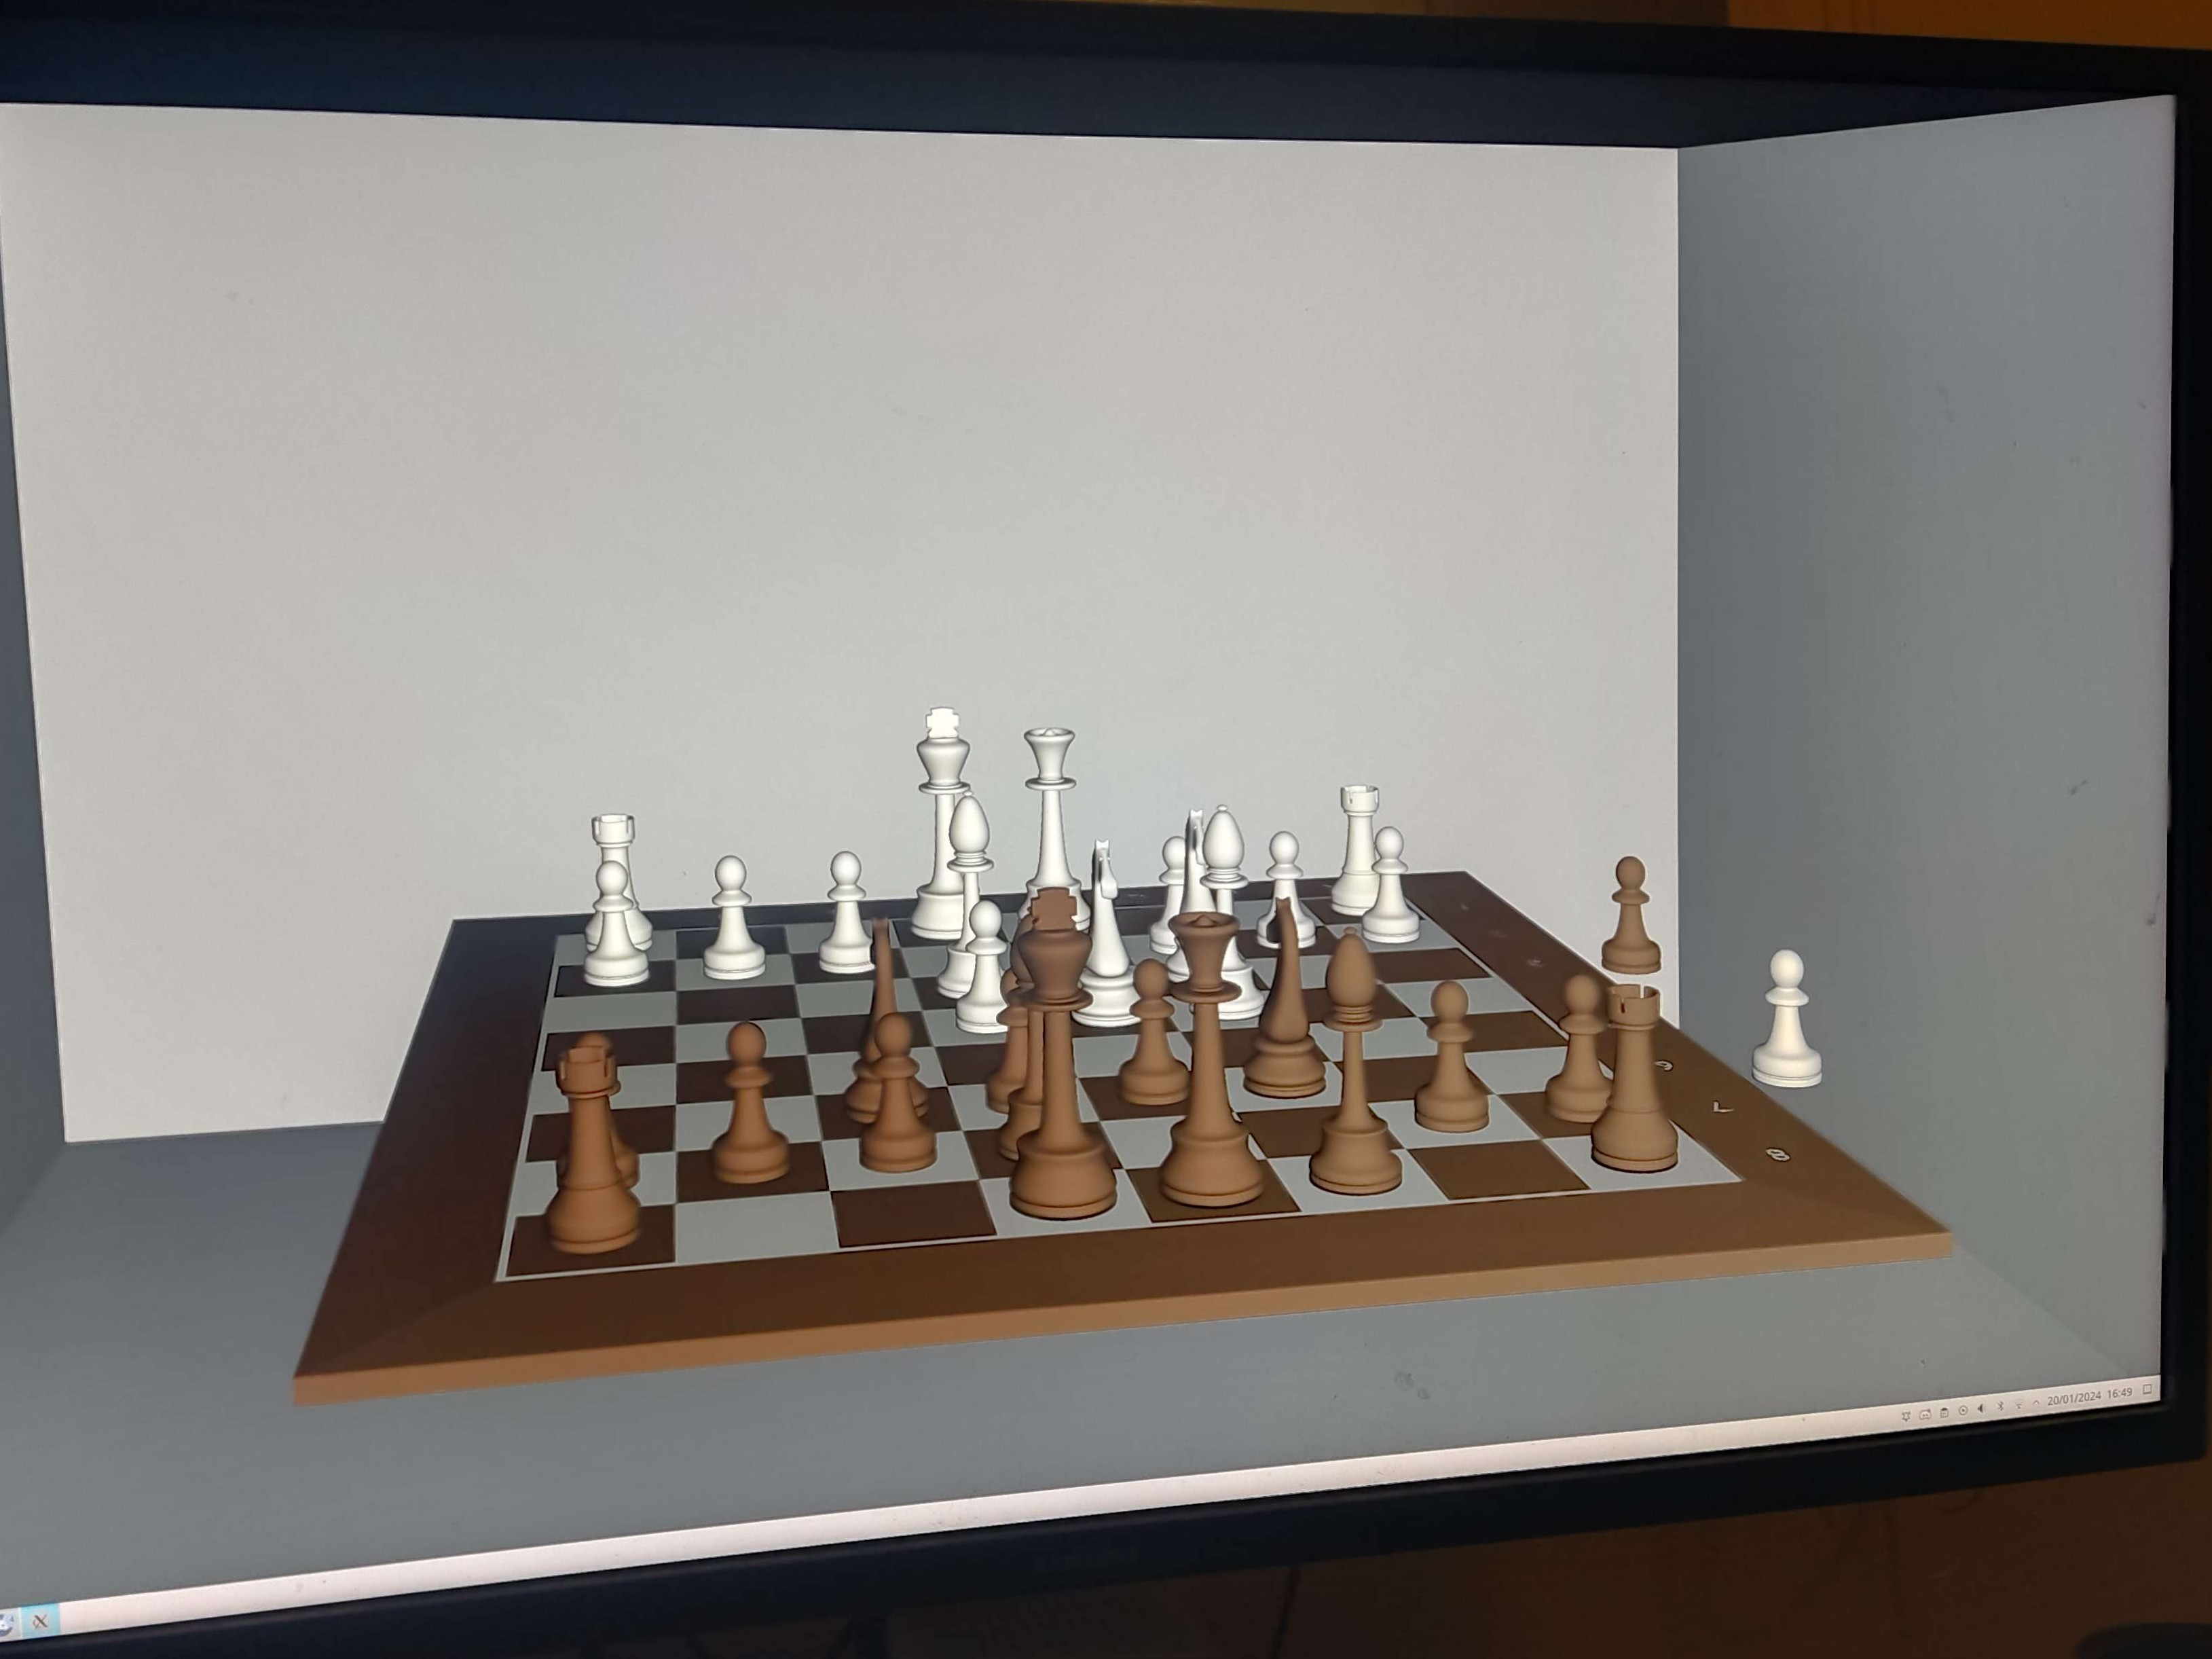
\includegraphics{./implementation/figures/perspective/left.jpg}
		}
	}
\end{invisBox}

\subsection{Object Loading}

Object loading support was added to the rendering system to facilitate the rendering of complex 3D models. We used the tinyobjloader library \cite{noauthor_tinyobjloadertinyobjloader_2024} to load \texttt{.obj} object files. We chose this library over alternatives like Assimp \cite{noauthor_assimpassimp_2024} due to its lightweight nature. We constructed our challenge for the user study by modifying primitives such as spheres, cylinders, and cubes loaded as \texttt{.obj} files using tinyobjloader to create an interactive task for the user.

\subsection{Lighting}

As shadows enhance the illusion of depth \cite{Kersten1997-xq}, we added a simple lighting model to the scene. We employed the Blinn-Phong \cite{10.1145/563858.563893} lighting model, which uses ambient, diffuse, and specular lighting. A comparison of the scene with and without lighting can be seen with the Erato Model \cite{McGuire2017Data} in Fig.~\ref{fig:erato} and Fig.~\ref{fig:erato-shadow}, respectively.

\begin{invisBox}
	\pictureBox[label={fig:erato}]{Erato}{
		\adjustbox{height=6.0cm, keepaspectratio}{
			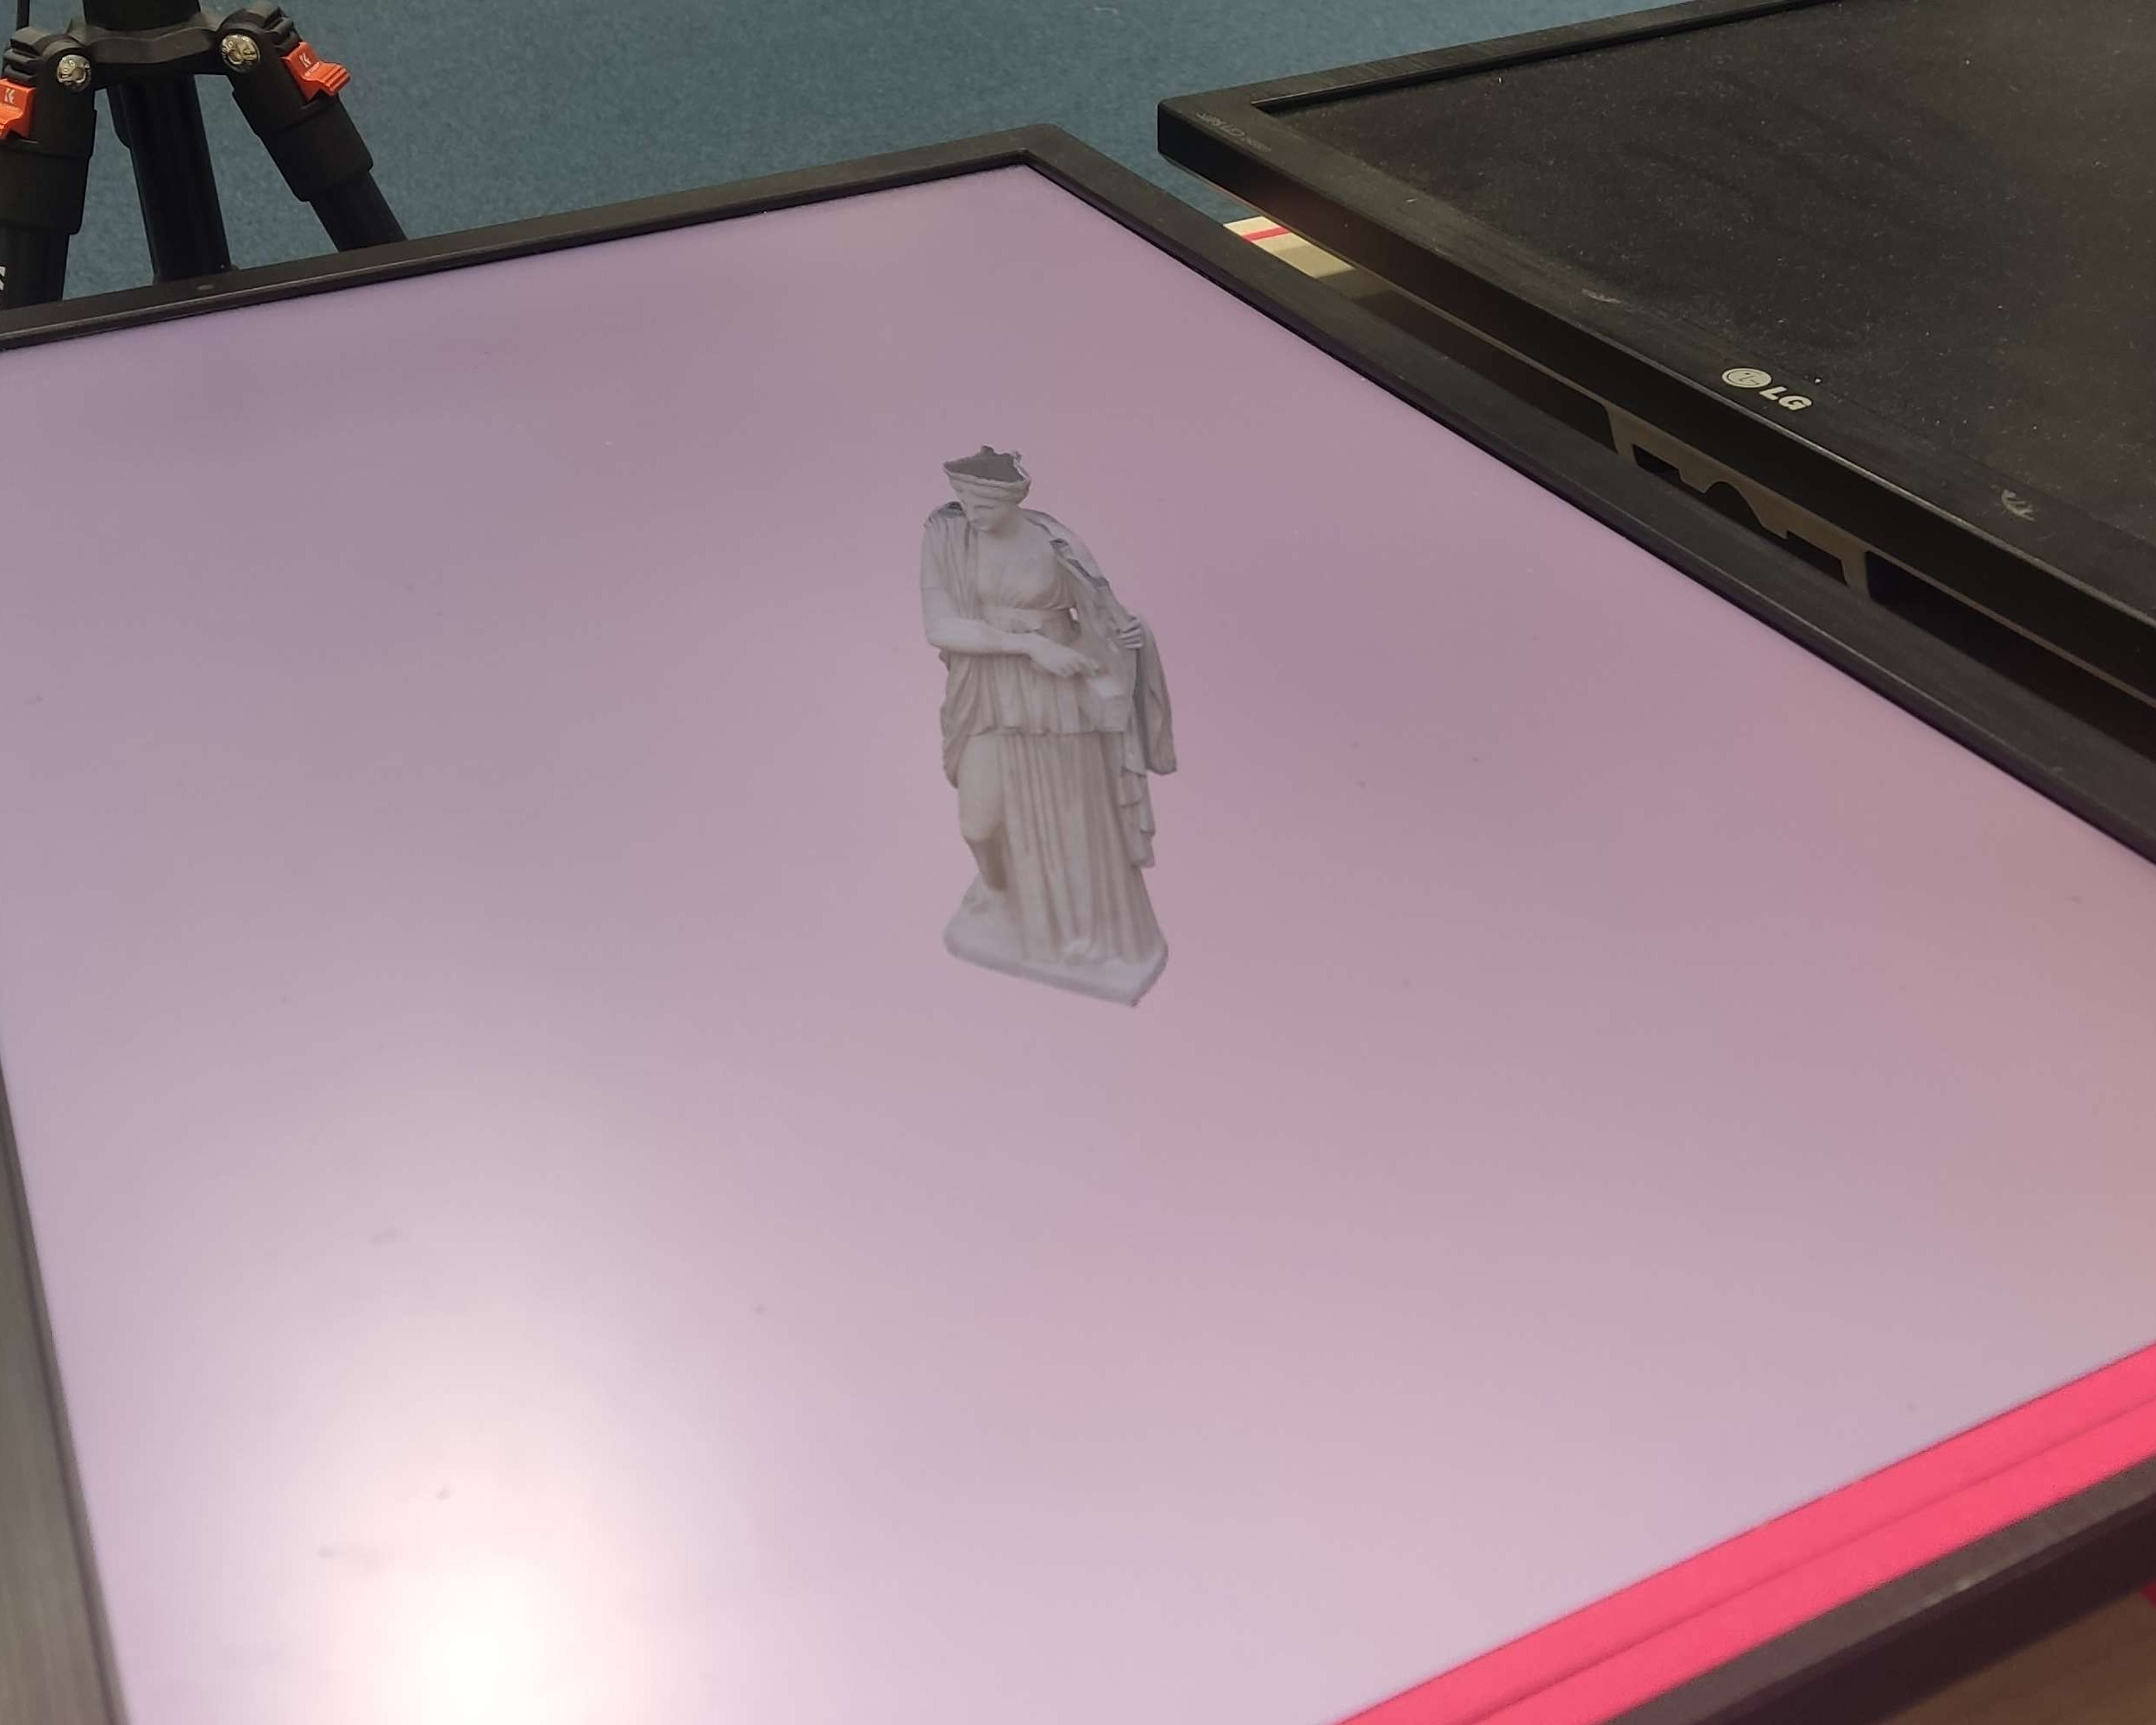
\includegraphics{./implementation/figures/perspective/erato.jpg}
		}
	}
	\hfill
	\pictureBox[label={fig:erato-shadow}]{Erato With Shadows}{
		\adjustbox{height=6.0cm, keepaspectratio}{
			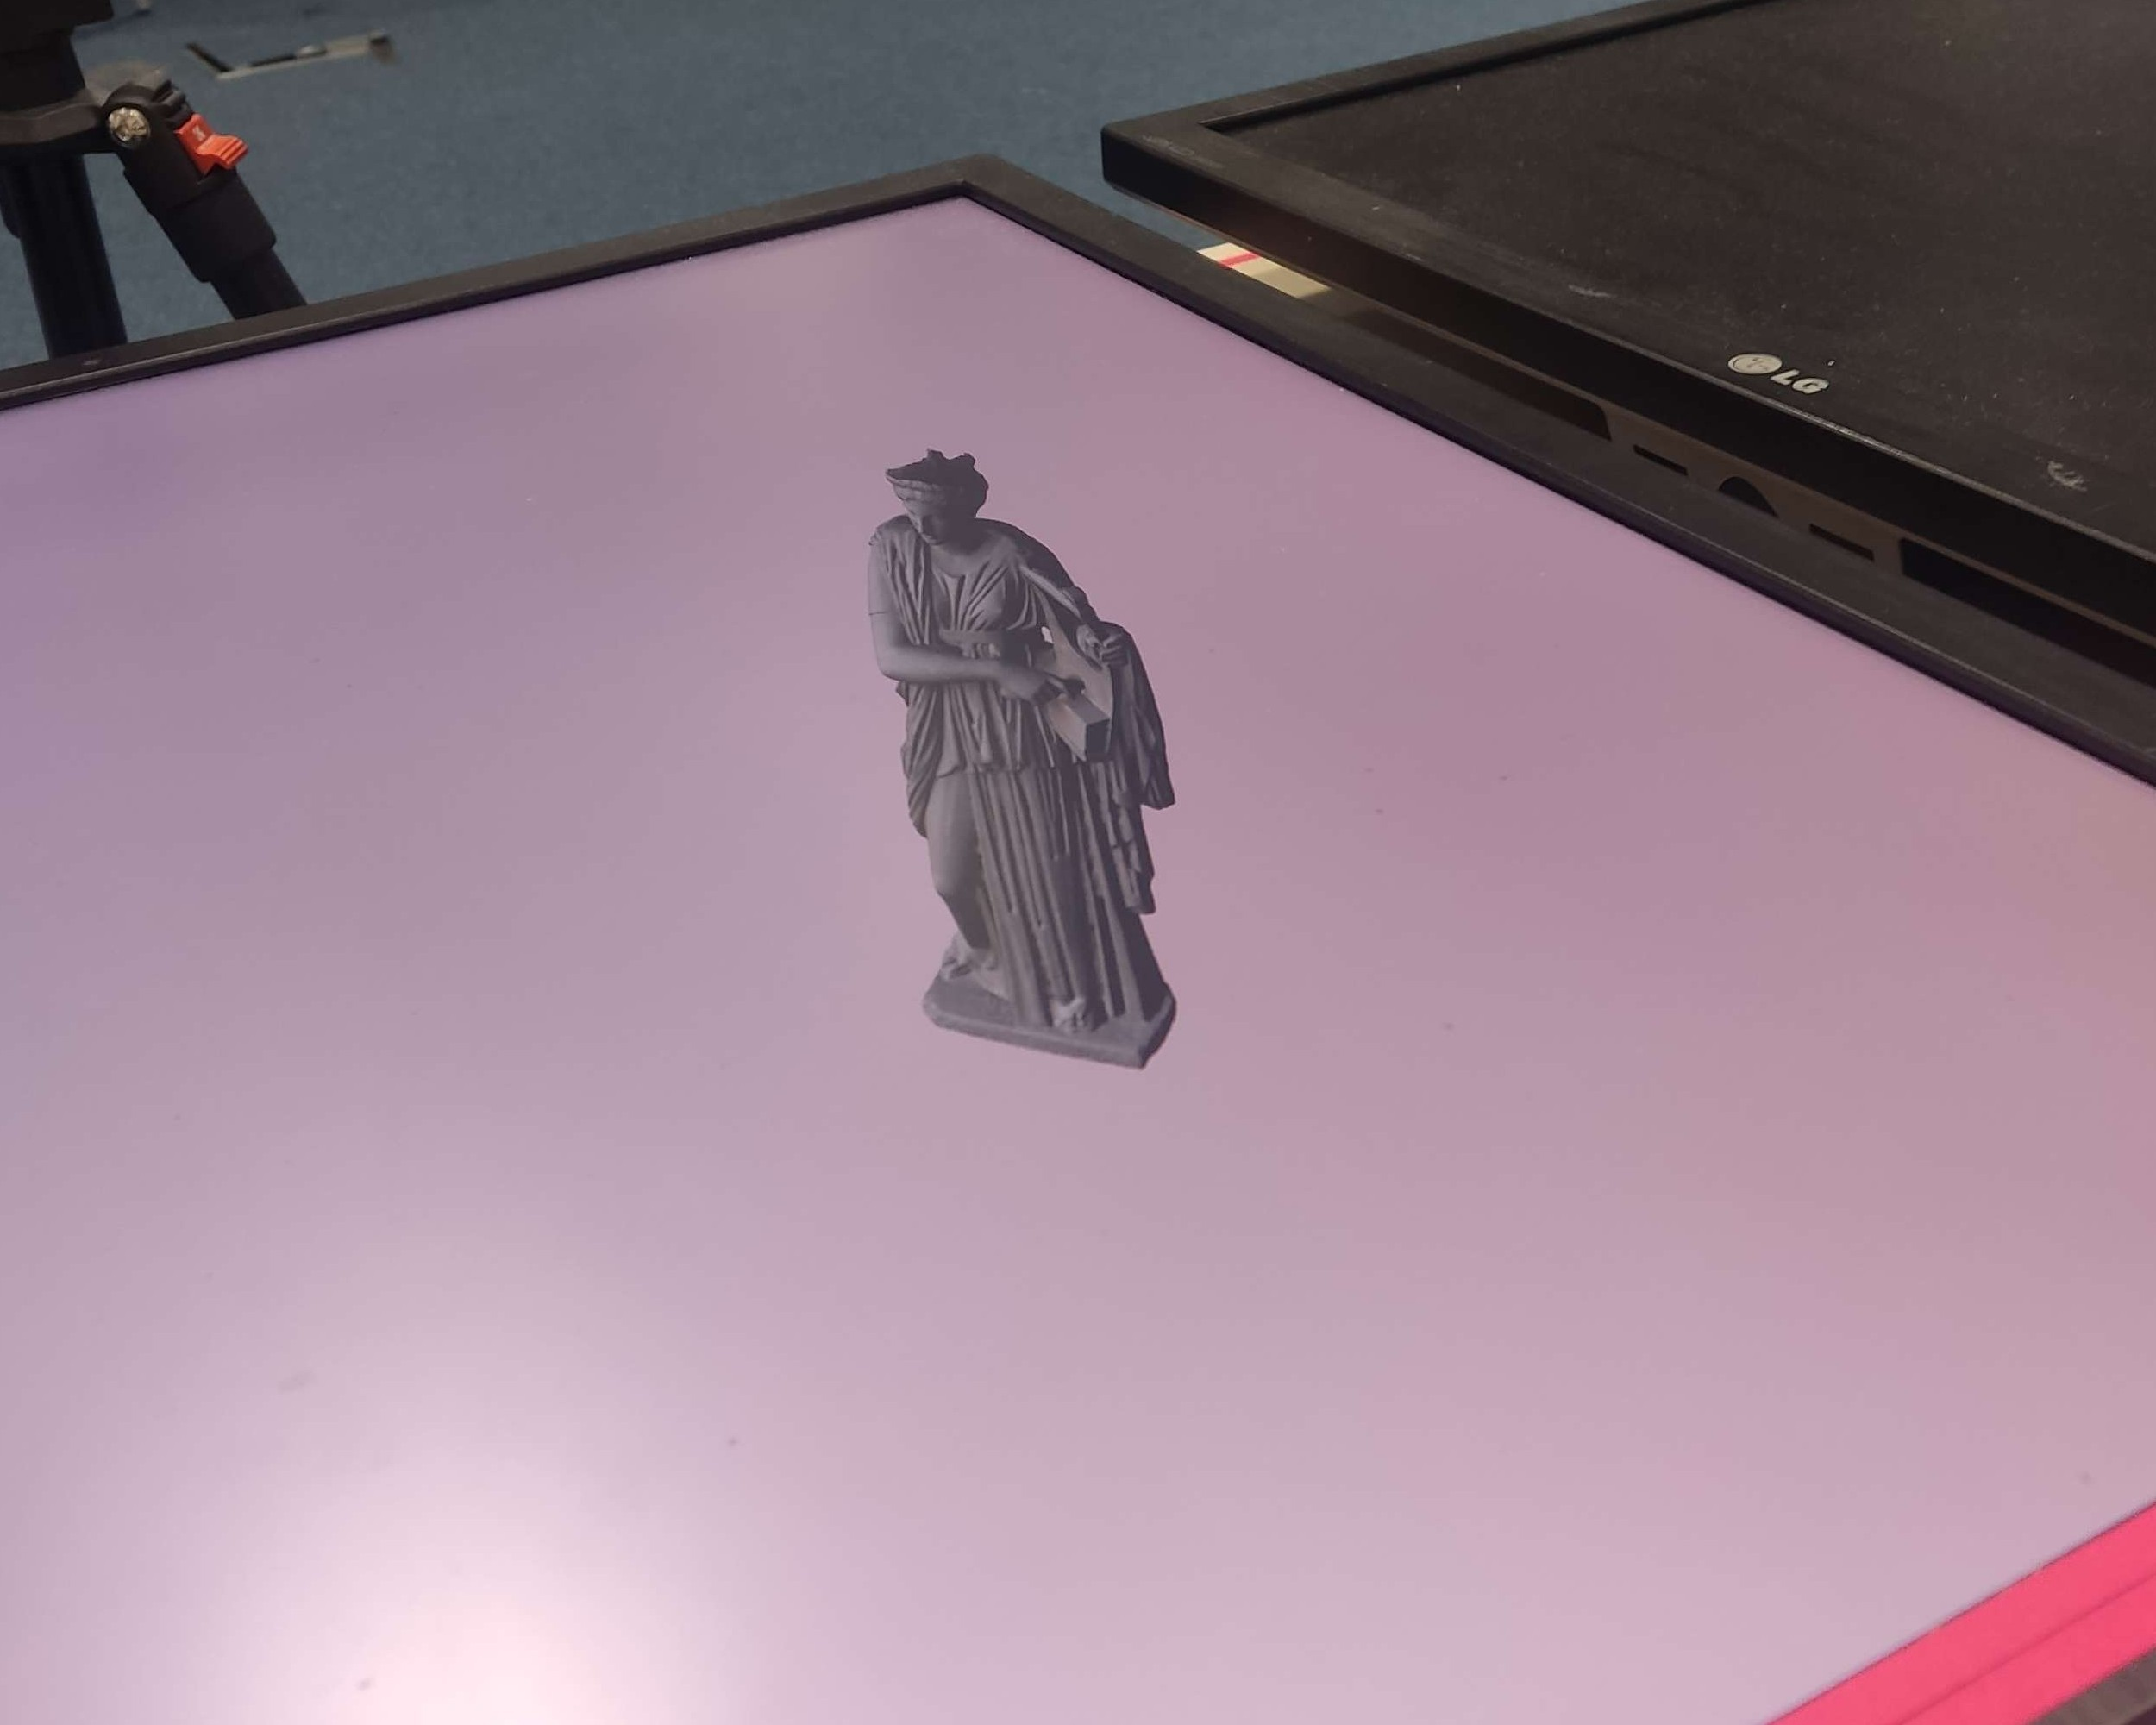
\includegraphics{./implementation/figures/perspective/erato_shadow.jpg}
		}
	}
\end{invisBox}
